\documentclass[11pt,a4paper]{article}
\usepackage[margin=2.2cm]{geometry}
\usepackage{amsmath,amssymb}
\usepackage{graphicx}
\usepackage{booktabs}
\usepackage{float}
\usepackage{xcolor}
\usepackage{enumitem}
\usepackage{caption}
\usepackage{array}
\usepackage{adjustbox}
\usepackage{microtype}
\usepackage{xurl}
\usepackage[colorlinks=true,linkcolor=blue!50!black,urlcolor=blue!60!black,citecolor=blue!50!black]{hyperref}
\setlength{\emergencystretch}{2em}
\setlist{itemsep=2pt,topsep=3pt}
\captionsetup{font=small}
\newcommand{\repourl}{https://github.com/usama-azam/DLSTG-PA3}
\newcommand{\kaggleurl}{https://www.kaggle.com/code/usamaazam9/dlstg-pa3-largest-sd-stgnn}

\begin{document}
% ---------------------------------------------------------------------------
\begin{titlepage}
\centering
{\large Lahore University of Management Sciences\\School of Science and Engineering, Department of Artificial Intelligence\par}
\vspace{1.2cm}
{\LARGE\bfseries AI651 -- Deep Learning for Space, Time and Graphs\par}
\vspace{0.4cm}
{\Large Programming Assignment 3\par}
\vspace{0.3cm}
{\large Spatio-Temporal Traffic Forecasting on LargeST-SD\\with Fixed, Adaptive and Hybrid Graphs\par}
\vspace{1.5cm}
{\Large Usama Azam\par}
{\large Roll No.\ 25280109\par}
\vspace{1.0cm}
{\textbf{GitHub repository}\\[2pt] \url{\repourl}\par}
\vspace{0.4cm}
{\textbf{Kaggle notebook (executed run)}\\[2pt] \small\url{\kaggleurl}\par}
\vspace{1.2cm}

\begin{minipage}{0.86\linewidth}
\small
\textbf{Summary.} Questions 1--2 are answered analytically and every claim is checked numerically in the notebook.
For Questions 3--7 we extract the 716 San Diego sensors of LargeST for 2020--2021, aggregate the 5-minute
vehicle counts to 15-minute totals, and train a lightweight temporal-convolution + graph-convolution model
(8 steps in, 4 steps out) under one protocol with four graph choices. On the April--December 2021 test period
(all values in vehicles per 15 minutes) the test MAE is: temporal-only 64.23, fixed road graph 58.88, learned
adaptive graph 51.34, hybrid graph 51.43. The learned graph overlaps the road graph only slightly more than random
pairs do: it links sensors with similar flow profiles rather than nearby sensors.
\end{minipage}
\vfill
{\small Fall 2026 \quad$\cdot$\quad Submitted November 2026}
\end{titlepage}

\tableofcontents
\newpage

% ---------------------------------------------------------------------------
\section{Question 1 -- What does a sum remember?}
All numerical claims below are verified by brute force in Part Q1 of the notebook.

\subsection*{(a) Affine message}
With $\phi(x)=wx+c$,
\[
  \sum_{u\in N(v)}\phi(x_u)=\sum_{u\in N(v)}(wx_u+c)=w\,S_v+c\,n_v ,
  \qquad h_v=\rho\big(wS_v+c\,n_v\big).
\]
The aggregated message is a function of the pair $(n_v,S_v)$ only, and $\rho$ sees nothing else. Hence two
neighbourhoods with the same $n_v$ and $S_v$ produce the \emph{same} input to $\rho$ and therefore the same
$h_v$, whatever $w$, $c$ and $\rho$ are. Example: $N_1=\{-1,+1,0\}$ and $N_2=\{0,0,0\}$ both have
$n_v=3$, $S_v=0$, but contain one and three steady neighbours respectively. Because a slowing and a speeding-up
neighbour cancel in $S_v$, the affine layer cannot tell ``one slowing + one speeding'' from ``two steady''. The
notebook confirms identical outputs for random $(w,c)$ and a nonlinear $\rho$.

\subsection*{(b) A nonlinear scalar message that stores all three counts}
Let $n_-,n_0,n_+$ be the numbers of slowing, steady and speeding-up neighbours, with
$1\le n_-+n_0+n_+\le K$. Each count is at most $K$, i.e.\ a digit in base $B=K+1$. Choose
\[
  \phi(-1)=1,\qquad \phi(0)=K+1,\qquad \phi(+1)=(K+1)^2 .
\]
Then $s=\sum_{u}\phi(x_u)=n_-+n_0(K+1)+n_+(K+1)^2$, which is exactly the base-$(K+1)$ number with digits
$(n_+,n_0,n_-)$. Because every digit is $\le K<K+1$, no carry can occur, so the representation is unique.
Decoding:
\[
  n_-=s \bmod (K+1),\qquad n_0=\Big\lfloor \tfrac{s}{K+1}\Big\rfloor \bmod (K+1),\qquad
  n_+=\Big\lfloor \tfrac{s}{(K+1)^2}\Big\rfloor .
\]
A smaller base fails: with base $K$, $K$ slowing neighbours give $s=K=\phi(0)$, the same as one steady neighbour.
For $K=8$ ($B=9$, $\phi=(1,9,81)$) the notebook enumerates all $164$ count triples with $1\le$ total $\le 8$, builds
every neighbourhood, sums the messages and checks that (i) all $164$ sums are distinct and (ii) the decoder
recovers every triple exactly. Both checks pass; e.g.\ $(n_-,n_0,n_+)=(2,1,3)\mapsto 2+9+243=254$.

\emph{Counting non-steady neighbours.} Take $\phi(x)=x^2$ (equivalently $|x|$): $\phi(\pm1)=1$, $\phi(0)=0$,
so $\sum_u\phi(x_u)=n_-+n_+$ for any neighbourhood size (also verified).

\subsection*{(c) Sum, mean and max with one-hot messages}
Write the aggregated vectors as $\mathbf s=(n_-,n_0,n_+)$ (sum), $\mathbf m=\mathbf s/n$ (mean) and
$\mathbf M=(\mathbb 1[n_->0],\mathbb 1[n_0>0],\mathbb 1[n_+>0])$ (max). The table was also confirmed by
enumerating all $164$ neighbourhoods of size 1--8 and searching for collisions.

\begin{center}
\small
\begin{tabular}{p{3.0cm}lcp{8.6cm}}
\toprule
Task & Method & Possible? & Reason \\
\midrule
(i) Count steady & Sum & Yes & $\rho$ reads coordinate 2: $n_0=s_2$. \\
 & Mean & No & $\{0\}$ and $\{0,0\}$ both give $\mathbf m=(0,1,0)$; answers $1$ vs $2$. \\
 & Max & No & $\{0\}$ and $\{0,0\}$ both give $\mathbf M=(0,1,0)$; answers $1$ vs $2$. \\
\midrule
(ii) More than half slowing & Sum & Yes & $n=s_1+s_2+s_3$; answer $=\mathbb 1[s_1>s_2+s_3]$ (i.e.\ $2s_1>n$). \\
 & Mean & Yes & coordinate 1 is the fraction slowing: answer $=\mathbb 1[m_1>\tfrac12]$. \\
 & Max & No & $\{-1,0\}$ and $\{-1,-1,0\}$ both give $\mathbf M=(1,1,0)$; answers No ($1/2$) vs Yes ($2/3$). \\
\midrule
(iii) Any slowing & Sum & Yes & answer $=\mathbb 1[s_1>0]$. \\
 & Mean & Yes & answer $=\mathbb 1[m_1>0]$ (since $m_1=n_-/n$ and $n\ge1$). \\
 & Max & Yes & answer $=M_1$. \\
\bottomrule
\end{tabular}
\end{center}
Sum is the most expressive aggregator (it keeps the multiset counts), mean keeps only proportions (loses $n$),
and max keeps only which trends are present (loses multiplicities), which is why it still detects ``any''.

% ---------------------------------------------------------------------------
\section{Question 2 -- Which way is the slowdown moving?}

\subsection*{(a)(i) Least-squares fit of the symmetric layer}
With $x_{20}(t)=1$ and all other readings 0, the only nonzero predictions are
$\hat x_{19}=b$, $\hat x_{20}=a$, $\hat x_{21}=b$, while the correct next snapshot is
$x_{19}=1$, $x_{20}=0$, $x_{21}=0$. Hence
\[
  L(a,b)=(b-1)^2+a^2+b^2,\qquad
  \frac{\partial L}{\partial a}=2a=0,\qquad \frac{\partial L}{\partial b}=2(b-1)+2b=0
  \;\Rightarrow\; a=0,\; b=\tfrac12,\; L_{\min}=\tfrac12 .
\]
Sensors 19 and 21 receive identical inputs (one neighbour equal to 1), so they must receive the same
prediction; the best compromise splits the slowdown equally. \texttt{np.linalg.lstsq} returns the same
$a=0,\ b=0.5$, SSE $=0.5$.

\subsection*{(a)(ii) Rolling the fitted layer forward}
Figure~\ref{fig:q2} shows the true motion and the 20-step autoregressive roll-out of $\hat x_i(t+1)=\tfrac12(x_{i-1}+x_{i+1})$
on the bump $x_i(0)=e^{-(i-20)^2/8}$ (same colour scale). The true bump translates one sensor per step without changing shape (its peak
reaches sensor 0 at $t=20$ and wraps round the ring). The symmetric layer never moves the bump: its peak stays at
sensor 20 while it spreads out and flattens (peak $1\to\approx0.40$ at $t=20$, total mass conserved). It
is a diffusion operator rather than a transport operator.

\begin{figure}[h]
  \centering
  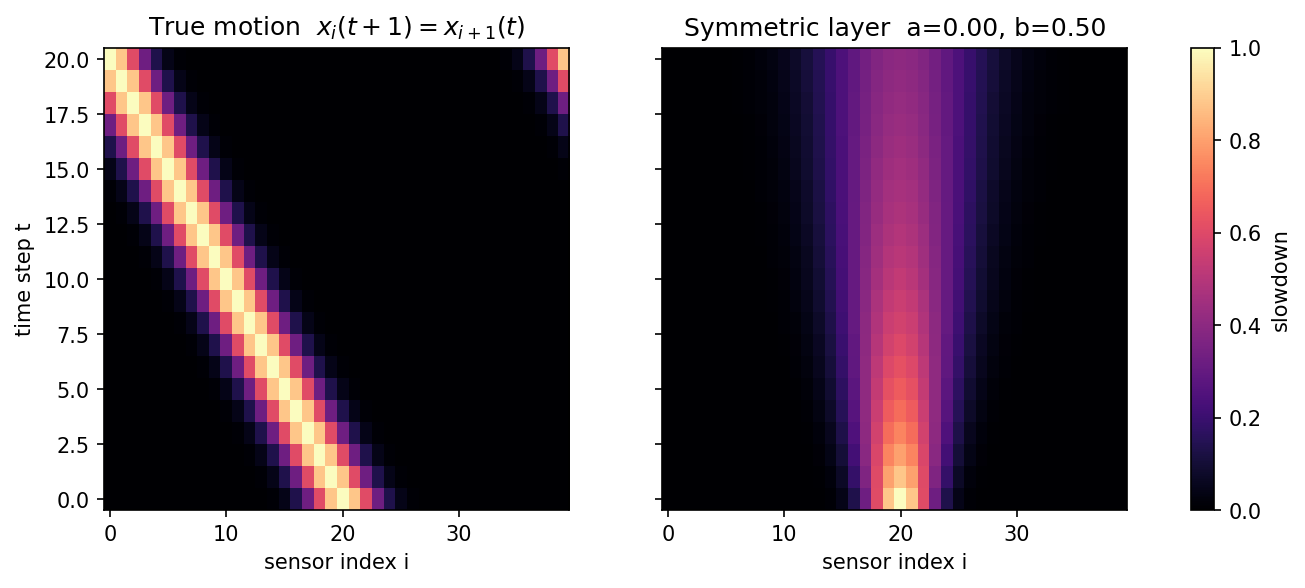
\includegraphics[width=0.82\linewidth]{figures/q2a_heatmaps.png}
  \caption{Q2(a)(ii): true backward motion (left) versus the fitted symmetric layer applied recursively (right).}
  \label{fig:q2}
\end{figure}

\subsection*{(b) Direction-aware weights}
Choose $a=0,\ w_-=0,\ w_+=1$. Substituting,
$\hat x_i(t+1)=0\cdot x_i(t)+0\cdot x_{i-1}(t)+1\cdot x_{i+1}(t)=x_{i+1}(t)=x_i(t+1)$ for every input and
every $i$ (indices mod 40), so the prediction is exact. Because the layer now knows which neighbour is
\emph{ahead} and which is \emph{behind}, the mirror symmetry $i\mapsto 40-i$ that forced $\hat x_{19}=\hat x_{21}$ in
(a) is broken. The layer can copy from the ahead neighbour only, which is exactly the motion rule.

\emph{As a 1-D convolution.} In PyTorch-style cross-correlation, the kernel entries that multiply
$[x_{i-1},x_i,x_{i+1}]$ are $[w_-,a,w_+]=[0,0,1]$. The ring is handled with \textbf{circular padding} of one
sensor on each side (\texttt{F.pad(x,(1,1),mode="circular")}, or \texttt{padding\_mode="circular"} in
\texttt{nn.Conv1d}), so sensor 39 sees sensor 0 as its ahead neighbour. The notebook confirms that this
convolution equals \texttt{np.roll(x,-1)} on random inputs.

\subsection*{(c) History with equal neighbour weights}
\textbf{(i) Backward motion.} The rule $x_i(t)=x_{i+1}(t-1)$ gives $x_{i-1}(t)=x_i(t-1)$: the reading that was at
sensor $i$ has moved to sensor $i-1$. The target is $x_i(t+1)=x_{i+1}(t)$. Choose $a=0,\ b=1,\ c=-1$:
\[
  \hat x_i(t+1)=x_{i-1}(t)+x_{i+1}(t)-x_i(t-1)=x_{i-1}(t)+x_{i+1}(t)-x_{i-1}(t)=x_{i+1}(t)=x_i(t+1). \checkmark
\]
\textbf{(ii) Forward motion} $x_i(t+1)=x_{i-1}(t)$. Now $x_i(t-1)=x_{i+1}(t)$ (the old reading at $i$ moved
forward to $i+1$), and with the same coefficients
\[
  \hat x_i(t+1)=x_{i-1}(t)+x_{i+1}(t)-x_i(t-1)=x_{i-1}(t)+x_{i+1}(t)-x_{i+1}(t)=x_{i-1}(t)=x_i(t+1). \checkmark
\]
The same coefficients are exact for both directions; the notebook checks both on 200 random patterns
(maximum error $4\times10^{-16}$).

\textbf{(iii) Why history helps.} The previous reading $x_i(t-1)$ equals the current reading of whichever
neighbour the pattern has just moved \emph{into}, i.e.\ the neighbour that holds information which has already
passed sensor $i$. Subtracting it cancels that neighbour from the symmetric sum and leaves the neighbour whose
reading is about to arrive. The direction is therefore read from the data (the pair
$(\mathbf x(t-1),\mathbf x(t))$ encodes the velocity), not from asymmetric weights. In effect the layer is the
leapfrog discretisation of the wave equation, $x(t+1)-2x(t)+x(t-1)=x_{i+1}-2x_i+x_{i-1}$, whose solutions move
in either direction depending on the initial velocity. For traffic models this means temporal context can
supply directional information that an undirected graph convolution alone cannot.


% ---------------------------------------------------------------------------
\section{Question 3 -- Dataset preparation and graph construction}

\subsection{Q3(a) Extraction, resampling and missing values}
\paragraph{Source and extraction.} We use the Kaggle copy of LargeST (\texttt{liuxu77/largest}). The files
\texttt{ca\_his\_raw\_2020.h5} and \texttt{ca\_his\_raw\_2021.h5} are pandas \emph{fixed-format} HDF5 tables
(timestamps $\times$ 8\,600 California sensors, float64, $\approx$7.2\,GB each). The 716 San Diego sensors
are the rows of \texttt{ca\_meta.csv} with \texttt{District}$=11$. Rather than load 7\,GB per year, we read
\texttt{block0\_values} with \texttt{h5py} in blocks of 8\,192 rows and keep only the San Diego columns, matched
by sensor ID (loading both years takes 67\,s). Each year is reindexed to a complete 5-minute grid (2020:
105\,408 steps, a leap year; 2021: 105\,120 steps).

\paragraph{Aggregation 5\,$\to$\,15 min.} LargeST inherits PeMS ``flow'', which is the number of vehicles
counted during each 5-minute interval, summed over lanes. Because this is an \emph{interval count}, we
\textbf{sum} three consecutive readings: $X^{15}_t=\sum_{k=0}^{2}X^{5}_{3t+k}$. The unit is therefore
\emph{vehicles per 15 minutes}. Averaging would instead give vehicles per 5 minutes, which is a factor of 3 smaller.
If only one or two of the three readings exist, we use $3\times$ their mean, which equals the sum when nothing is
missing and is otherwise an unbiased estimate. An interval with all three readings missing is marked missing. The
result is $X\in\mathbb R^{70\,176\times716\times1}$ (2020-01-01 00:00 to 2021-12-31 23:45).

\paragraph{Missing values.} 5.07\% of 5-minute readings are NaN (2020: 4.10\%, 2021: 6.03\%); only 0.02\% of
15-minute intervals are partially observed and 5.06\% are fully missing. Missingness is concentrated in a few
sensors: the median sensor misses 0.011\%, but 45 sensors miss more than 10\% and 19 sensors report nothing
at all (Figure~\ref{fig:q3a}, bottom). We handle missing data in two separate ways:
\begin{enumerate}
\item \textbf{Targets and metrics.} A mask records which 15-minute values were actually observed. The training
loss and every reported metric are computed \emph{only on observed targets} (masked MAE/RMSE), so imputed values
are never treated as ground truth.
\item \textbf{Model inputs.} Gaps of at most 1\,h (4 steps) are filled by linear interpolation in time (6\,818 values).
Longer gaps are filled with the sensor's \emph{2020 (training) time-of-week mean profile} (2.54\,M values, mostly the
dead sensors), falling back to the sensor's training mean or the global training mean. Only training-period
statistics are used, so no validation or test information leaks into the inputs.
\end{enumerate}

\begin{figure}[H]
  \centering
  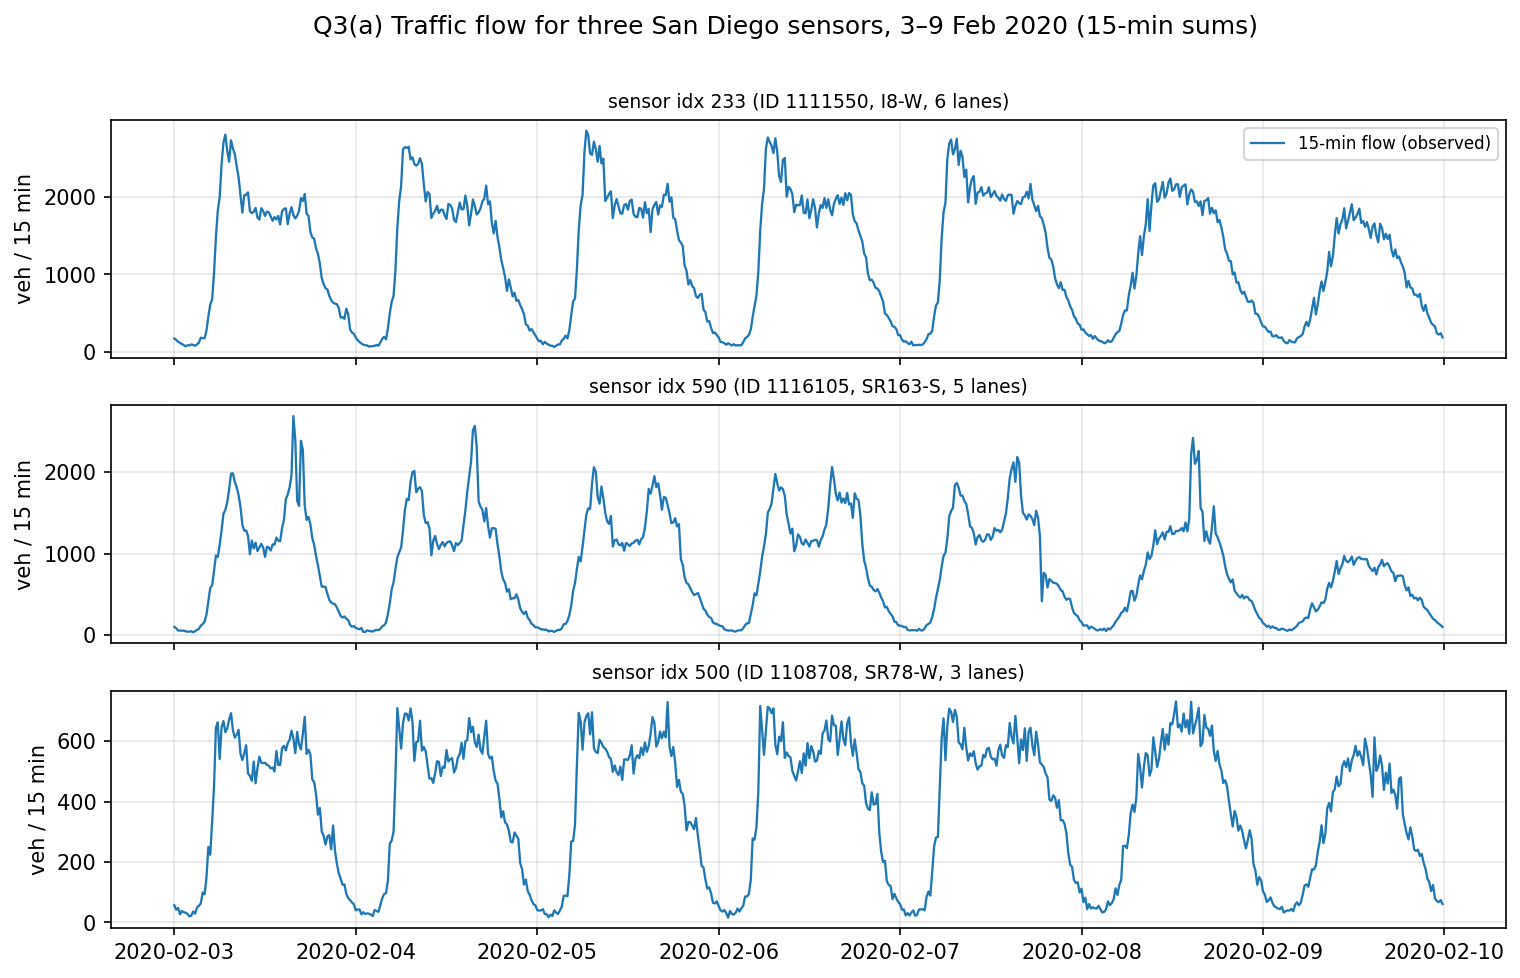
\includegraphics[width=0.93\linewidth]{figures/q3a_three_sensors_week.png}\\
  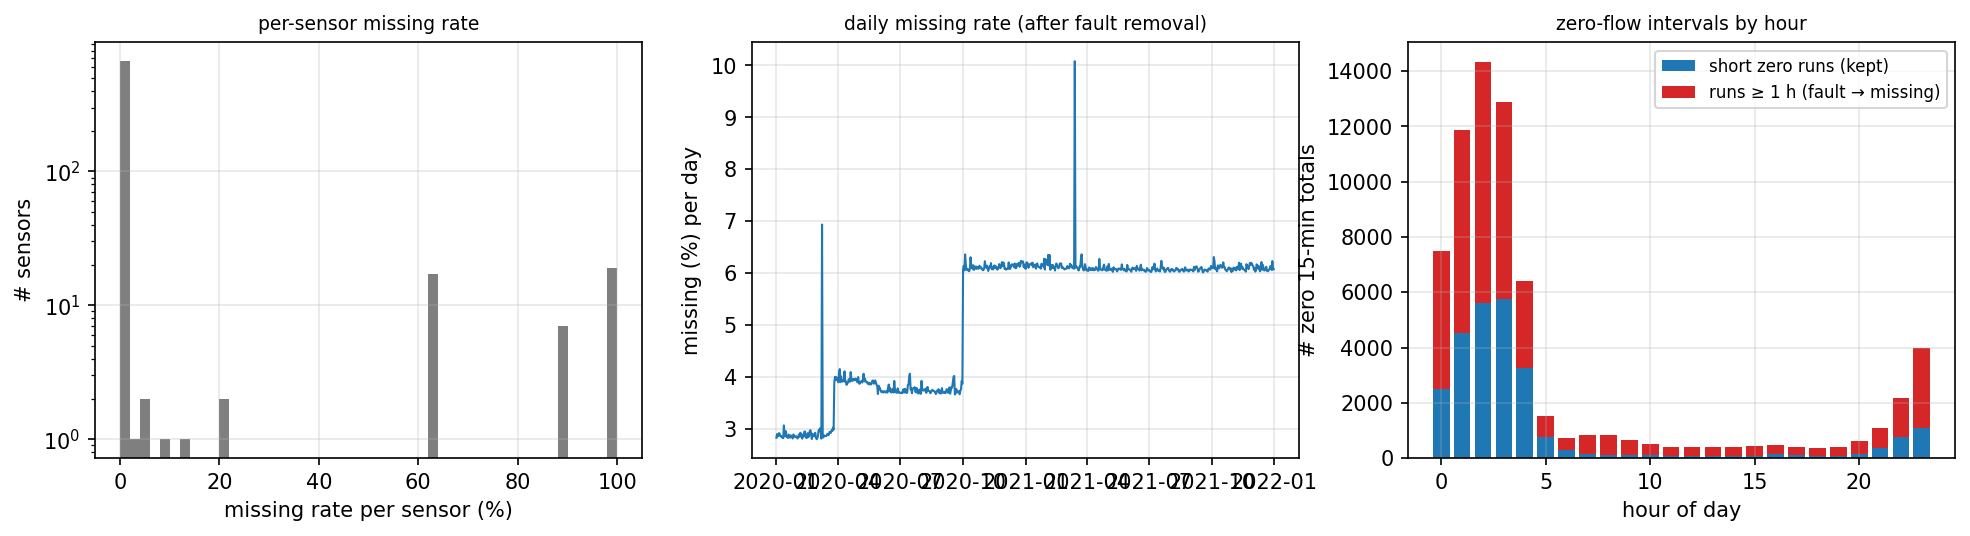
\includegraphics[width=0.85\linewidth]{figures/q3a_missing.png}
  \caption{Q3(a). Top: 15-minute flow of three sensors (high, median and low volume; all with $<2\%$ missing)
  during Mon 3 -- Sun 9 Feb 2020. The weekday morning and evening peaks and the lower, later weekend profile are
  clearly visible. Bottom: per-sensor missing rate (log scale) and daily missing percentage over 2020--2021.}
  \label{fig:q3a}
\end{figure}

\subsection{Q3(b) The road-distance graph}
\texttt{ca\_rn\_adj.npy} (8\,600$\times$8\,600) is indexed in the row order of \texttt{ca\_meta.csv}. The h5
columns follow the same order (the IDs match), and we take $A_{SD}=A[\text{sd},\text{sd}]$ with the same index
vector used for the traffic columns. Node $k$ of the graph is therefore column $k$ of the traffic tensor.

\begin{center}\small
\begin{tabular}{lr@{\hspace{2.2em}}lr}
\toprule
Nodes & 716 & Symmetric? & \textbf{No} \\
Nonzero entries (incl.\ self-loops) & 18\,035 & One-direction-only pairs ($i<j$) & 3\,711 \\
Self-loops ($A_{ii}=1$) & 716 & Off-diagonal weight range & $[0.01,\,1.00]$ \\
Directed edges ($i\ne j$) & 17\,319 & Out-degree mean/median/max & 24.2/20/70 \\
Undirected connected pairs & 10\,515 & Off-diagonal density & 3.38\% \\
\bottomrule
\end{tabular}
\end{center}

The matrix is \emph{directed}: road distance from $i$ to $j$ along the freeway network is not the distance from
$j$ to $i$, especially between the two carriageways of a freeway or at ramps and interchanges. The weights look
like a thresholded Gaussian kernel $A_{ij}=\exp(-d_{ij}^2/\sigma^2)$ with entries below $\approx0.01$ removed.
Three sensors have no edges at all.

\textbf{Meaning of $A_{ij}\neq0$.} Sensor $j$ can be reached from sensor $i$ within a short \emph{road-network}
distance $d_{ij}$, and the value (between 0 and 1) measures how close they are: 1 means essentially co-located,
and values near 0.01 mean at the edge of the kernel. It encodes proximity along roads, not straight-line
distance and not measured traffic correlation. In the GCN, row $i$ of $\hat A$ says which sensors node $i$
aggregates from and with what weights.

\begin{figure}[H]
  \centering
  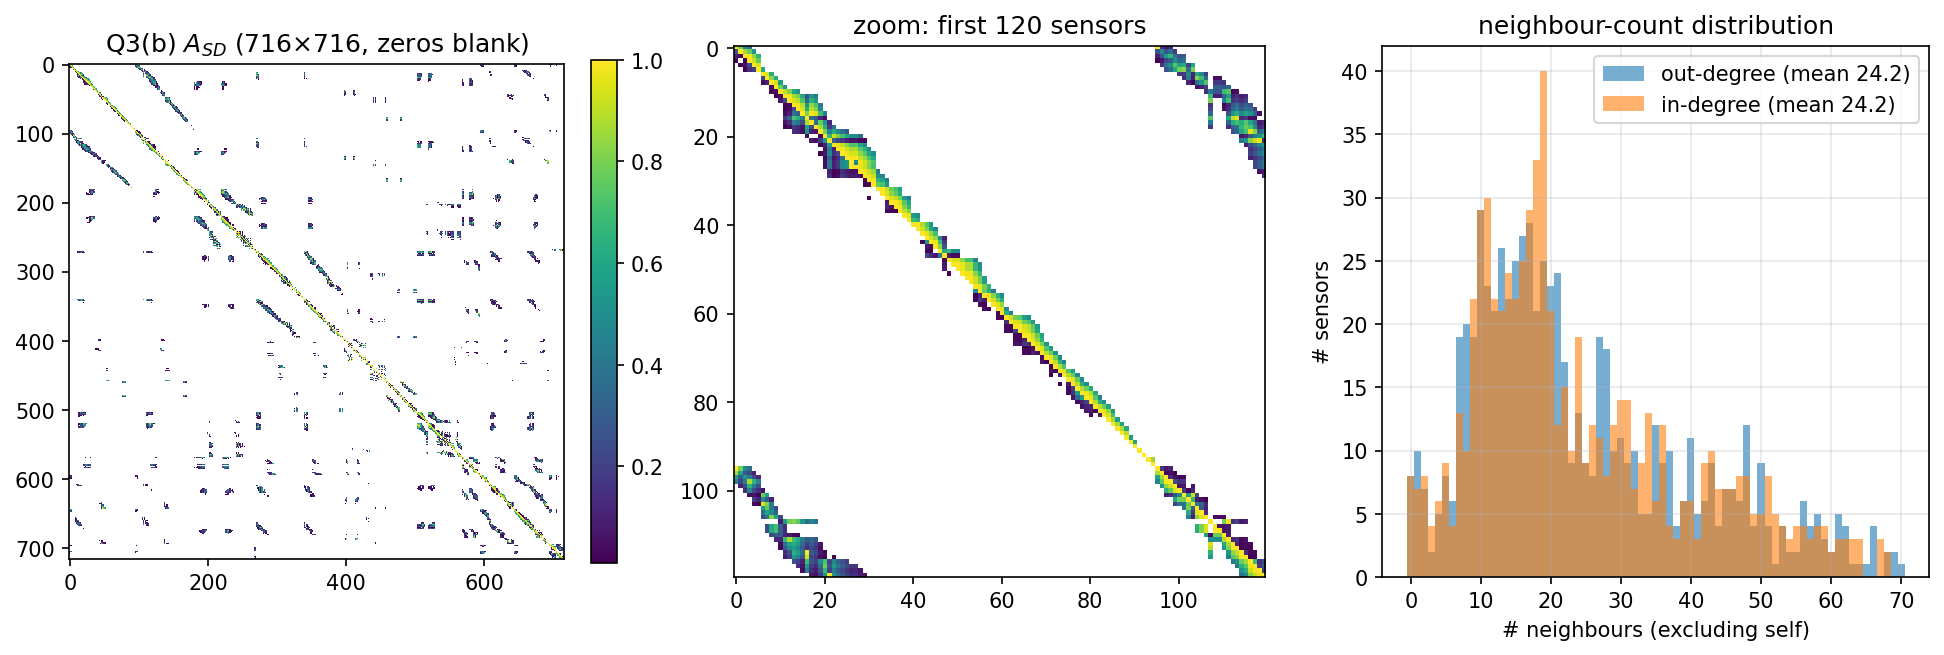
\includegraphics[width=\linewidth]{figures/q3b_adjacency.png}
  \caption{Q3(b). $A_{SD}$ heatmap (zeros blank), a zoom on the first 120 sensors, and the distribution of
  out-/in-degree (number of neighbours excluding self). The banded structure comes from consecutive sensor IDs along
  the same freeway; the off-diagonal blocks are interchanges and opposite carriageways.}
  \label{fig:q3b}
\end{figure}

\subsection{Q3(c) One-hop and two-hop neighbourhoods}
We picked a sensor with the median out-degree: \textbf{index 33, ID 1126411, I-5 North} (32.771$^\circ$N,
117.207$^\circ$W), close to the I-5/I-8 interchange. Its \textbf{one-hop} neighbourhood $\{j:A_{ij}\ne0,\,j\ne i\}$
has \textbf{20} sensors: 4 on I-5 N (weights 0.63--0.95, 2020 flow correlation 0.91--0.997), 7 on I-5 S, 6 on I-8 E and
3 on I-8 W (weights 0.01--0.46). Its \textbf{two-hop} neighbourhood (paths of at most two edges) has \textbf{73} sensors,
53 of which are reachable \emph{only} in two hops; these include sensors on SR-163 and I-805. Full ID lists are in the
notebook. Figure~\ref{fig:q3c} shows them on a map.

\begin{figure}[H]
  \centering
  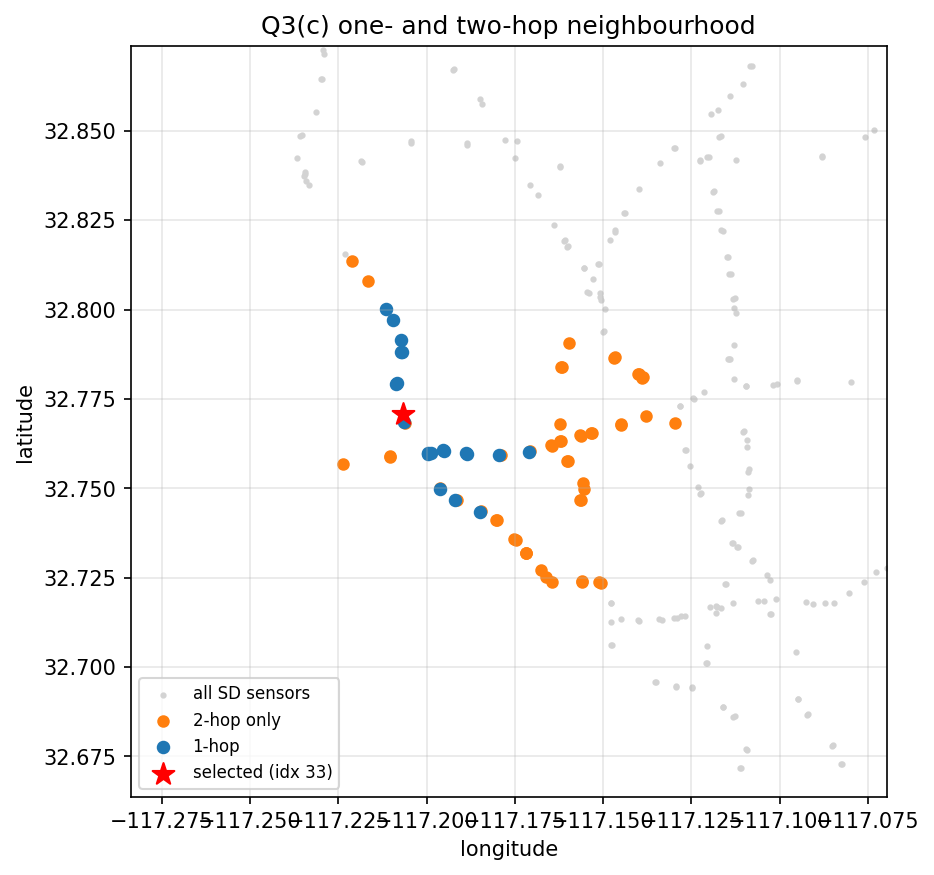
\includegraphics[width=0.48\linewidth]{figures/q3c_neighbourhood.png}
  \caption{Q3(c). Selected sensor (star), its 1-hop (blue) and 2-hop-only (orange) neighbours.}
  \label{fig:q3c}
\end{figure}

\begin{itemize}
\item \textbf{Why neighbours help.} Vehicles that pass sensor $i$ were recently at its upstream neighbours and will
soon reach its downstream ones. A shockwave or incident downstream propagates upstream within minutes. Neighbours on
the same carriageway are therefore leading indicators: in 2020 they correlate with the selected sensor at
$r=0.91$--$0.997$. Neighbours also provide redundancy when the sensor itself is noisy or missing.
\item \textbf{One-hop vs two-hop aggregation.} One graph-convolution layer ($\hat AZ$) mixes each node with its
direct neighbours only, here sensors within a few km. Two layers ($\hat A^2Z$) reach the 73-node two-hop set, which
spans several freeways around the interchange. Two-hop aggregation gives a wider receptive field (useful for
congestion arriving from further away or for longer horizons), but each extra hop also brings in nodes that are only
weakly related (correlations as low as 0.78 on I-805 S).
\item \textbf{Too many layers.} Yes. Repeated multiplication by a row-stochastic $\hat A$ is a diffusion: after $L$
layers every node averages an $L$-hop region (with a mean degree of 24 this soon covers the whole network), so
node representations converge toward one another (\emph{over-smoothing}) and lose the local detail needed to
forecast a single sensor. Deep GCNs also over-squash information from exponentially many nodes into a fixed-width
vector, are harder to optimise, and cost more. We use two residual layers: enough for two hops while the residual
keeps each node's own temporal features.
\end{itemize}

% ---------------------------------------------------------------------------
\section{Question 4 -- Spatio-temporal traffic forecasting}

\subsection{Q4(a) Windows, splits and normalisation}
For each $t$, $X_t=[x_{t-7},\dots,x_t]\in\mathbb R^{8\times716}$ and $Y_t=[x_{t+1},\dots,x_{t+4}]\in\mathbb R^{4\times716}$.
A window is assigned to a split only if all 12 of its time steps lie inside that split, so no window crosses a split
boundary.
\begin{center}\small
\begin{tabular}{lllr}
\toprule
Split & Period & First / last target time & \# windows \\
\midrule
Train & 1 Jan -- 31 Dec 2020 & 2020-01-01 02:00 / 2020-12-31 23:45 & 35\,125\\
Validation & 1 Jan -- 31 Mar 2021 & 2021-01-01 02:00 / 2021-03-31 23:45 & 8\,629\\
Test & 1 Apr -- 31 Dec 2021 & 2021-04-01 02:00 / 2021-12-31 23:45 & 26\,389\\
\bottomrule
\end{tabular}
\end{center}
Inputs and targets are z-scored with a single mean and standard deviation computed from \emph{observed 2020 values only}
($\mu=607.39$, $\sigma=483.77$ veh/15\,min). Predictions are de-normalised before computing metrics.

\subsection{Q4(b) Architecture}
\begin{itemize}
\item \textbf{Temporal encoder $f_{\text{temporal}}$} (weights shared by all sensors): each sensor's 8-step series is
passed through \texttt{Conv1d(1$\to$d, k=3)}, ReLU, \texttt{Conv1d(d$\to$d, k=3, dilation 2)}, ReLU. The receptive field
covers all 8 steps and the output has length 2. This is flattened and passed through \texttt{Linear(2d$\to$d)} and ReLU,
giving $Z\in\mathbb R^{B\times N\times d}$ with $d=32$.
\item \textbf{Spatial graph convolution:} $\mathrm{GC}(Z)=\mathrm{ReLU}(\hat A Z W_g)$. It is computed with
\texttt{torch.einsum} (subscripts \texttt{nm,bmd->bnd}), so the graph product acts on the node dimension
independently for each batch item.
We stack two such layers, each with a residual connection: $H^{(l+1)}=H^{(l)}+\mathrm{ReLU}(\hat A H^{(l)}W^{(l)})$, $H^{(0)}=Z$.
The residual means the graph model contains the temporal-only model as a special case, which keeps the comparison fair.
It also keeps a node's own signal when an adaptive $\hat A$ puts little weight on the diagonal.
\item \textbf{Forecast head $f_{\text{head}}$:} a per-node MLP \texttt{Linear(d$\to$d)}, ReLU, \texttt{Linear(d$\to$4)}, giving
$\hat Y\in\mathbb R^{B\times4\times N}$ (direct multi-horizon output).
\item \textbf{Loss:} masked MAE on normalised values (observed targets only).
\end{itemize}

\subsection{Q4(c) Temporal-only baseline}
The baseline uses the same encoder and head with the graph layers removed ($\hat Y=f_{\text{head}}(Z)$), and it is trained
with exactly the same protocol. Its results and the comparison are in Table~\ref{tab:main} and Section~\ref{sec:q6}.
In short, \textbf{explicit spatial modelling helps}. The fixed road graph lowers test MAE from 64.23 to 58.88
($-8.3\%$) and RMSE from 100.95 to 92.66 ($-8.2\%$). The gain grows with the horizon: at 15\,min it is $-4.3\%$ MAE and at
60\,min $-10.3\%$. A single sensor's last two hours say little about what will arrive in an hour, whereas upstream and
downstream sensors carry exactly that information.

% ---------------------------------------------------------------------------
\section{Question 5 -- Fixed versus learnable adjacency}
All three graph models share the encoder, two residual GC layers, head, data splits, seed (42), optimiser and
early-stopping rule. Only the graph module differs.

\subsection{Q5(a) Fixed adjacency}
Because $A_{SD}$ is directed, the symmetric $D^{-1/2}(A+I)D^{-1/2}$ does not apply. We use the \textbf{directed
random-walk normalisation}
\[
  \hat A=D^{-1}\tilde A,\qquad \tilde A=A\text{ with } \tilde A_{ii}=1,\qquad D_{ii}=\textstyle\sum_j\tilde A_{ij}.
\]
$A_{SD}$ already contains unit self-loops, so we set the diagonal to 1 instead of adding $I$, to avoid a double
self-loop. Each row of $\hat A$ sums to 1, so node $i$ takes a weighted \emph{average} of the nodes $j$ that it reaches
by road, and this works for any directed graph (no node has zero degree thanks to the self-loop). $\hat A$ is
registered as a non-trainable buffer and stays unchanged throughout training. Results: test MAE 58.88, RMSE 92.66,
training time 978\,s (Table~\ref{tab:main}).

\subsection{Q5(b) Learnable (adaptive) adjacency}
Two embedding matrices $E_1,E_2\in\mathbb R^{716\times10}$ ($d_e=10$) are \texttt{nn.Parameter}s initialised from
$\mathcal N(0,1)$. In every forward pass,
\[
  S=\mathrm{ReLU}(E_1E_2^\top),\qquad
  A_{\text{adaptive}}=\mathrm{Softmax}_{\text{row}}\big(\mathrm{TopK}_{k=20}(S)\big),
\]
where $\mathrm{TopK}$ keeps the 20 largest logits of each row and sets the rest to $-\infty$.
\begin{itemize}
\item \textbf{Sparsification is applied \emph{before} the normalisation.} After the softmax, each row is a probability
distribution over exactly its 20 kept neighbours (rows sum to 1, like the fixed $\hat A$). Applying top-$k$ \emph{after} a
dense softmax would leave rows that no longer sum to 1, with most of the mass thrown away while 716 nodes compete.
\item \textbf{Gradient flow.} The top-$k$ \emph{selection} is piecewise constant, so no gradient flows through the choice of
indices. In the backward pass it acts as a fixed mask. Gradients reach $E_1,E_2$ through the softmax and ReLU of the
\emph{kept} logits: $\partial S_{ij}/\partial E_{1,i}=E_{2,j}$ and $\partial S_{ij}/\partial E_{2,j}=E_{1,i}$ when
$S_{ij}>0$. Non-selected pairs get no gradient at that step, but because every embedding row is updated through its kept
pairs, the ranking changes during training and new neighbours can enter the top 20. The graph adds 14\,320 parameters
(22\,932 in total versus 8\,612 for the fixed model). It is learned only from training-window gradients, and the
validation set is used only for early stopping.
\end{itemize}
The learned matrix is shown in Figure~\ref{fig:adj} and analysed in Section~\ref{sec:q6b}. Compared with the fixed graph,
it lowers test MAE from 58.88 to \textbf{51.34} ($-12.8\%$) and RMSE from 92.66 to 81.17 ($-12.4\%$), at a cost of
+9\% training time.

\subsection{Q5(c) Hybrid adjacency}
\[
  A_{\text{hybrid}}=\alpha\,\hat A_{\text{fixed}}+(1-\alpha)\,A_{\text{adaptive}},\qquad \alpha=\sigma(a),\ a\in\mathbb R\ \text{learned},\ \alpha_0=0.5 .
\]
Both components are normalised consistently: both are \emph{row-stochastic} ($D^{-1}\tilde A$ and a row softmax), so
$A_{\text{hybrid}}$ is a convex combination and is row-stochastic too. The adaptive part uses its own embeddings with the
same top-20 rule. During training $\alpha$ fell from 0.50 to \textbf{0.057}: the model chose to rely mostly on the learned
graph and keep a small physical prior. The hybrid reaches test MAE 51.43 / RMSE 81.39, essentially the same as the
adaptive graph (difference $<0.2\%$). It is marginally better at the 45 and 60-minute horizons and marginally worse at
15 and 30 minutes.

\begin{figure}[H]
  \centering
  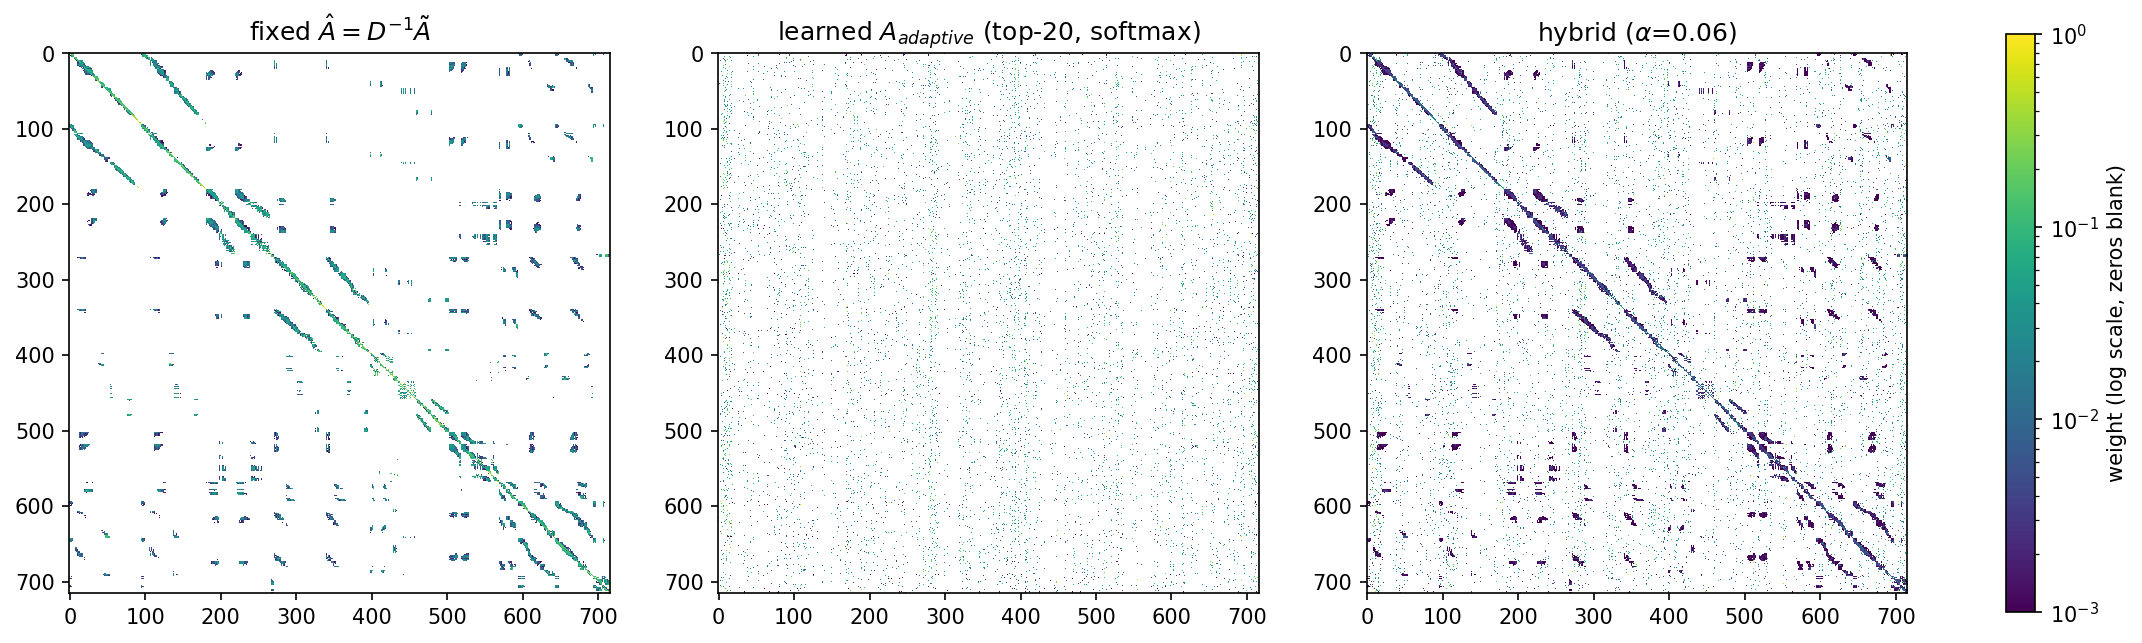
\includegraphics[width=\linewidth]{figures/q5_adjacency_fixed_adaptive_hybrid.png}
  \caption{Q5. Fixed $\hat A=D^{-1}\tilde A$ (left), learned top-20 $A_{\text{adaptive}}$ (centre) and hybrid with learned
  $\alpha=0.06$ (right); log colour scale, zeros blank. The road graph is banded (sensors along a freeway); the learned
  graph is spread over the whole matrix with a few vertical stripes (``hub'' columns that many sensors read from).}
  \label{fig:adj}
\end{figure}

% ---------------------------------------------------------------------------
\section{Question 6 -- Experimental analysis and interpretation}\label{sec:q6}

\subsection{Q6(a) Forecasting comparison}
\begin{table}[H]
\centering\small
\caption{Main results. Metrics in vehicles per 15 minutes, averaged over the 4 horizons and over all observed
(sensor, time) targets. Training time is the wall-clock time of the full training loop (including per-epoch validation)
on one Tesla T4.}
\label{tab:main}
\setlength{\tabcolsep}{4.5pt}
\begin{adjustbox}{max width=\linewidth}
\begin{tabular}{llrrrrrr}
\toprule
 & & \multicolumn{2}{c}{Validation} & \multicolumn{2}{c}{\textbf{Test}} & Training & Epochs \\
\cmidrule(lr){3-4}\cmidrule(lr){5-6}
Model & Adjacency & MAE & RMSE & \textbf{MAE} & \textbf{RMSE} & time & (best) \\
\midrule
Temporal-only & None     & 55.72 & 89.61 & 64.23 & 100.95 & 842\,s & 47 (39)\\
STGNN         & Fixed    & 50.06 & 80.63 & 58.88 & 92.66  & 978\,s & 49 (41)\\
STGNN         & Adaptive & \textbf{42.14} & \textbf{68.10} & \textbf{51.34} & \textbf{81.17} & 1063\,s & 50 (49)\\
STGNN         & Hybrid   & 42.33 & 68.75 & 51.43 & 81.39  & 1067\,s & 50 (42)\\
\midrule
\multicolumn{4}{l}{\emph{Reference: last value}} & 87.14 & 132.99 & -- & --\\
\multicolumn{4}{l}{\emph{Reference: 2020 time-of-week mean}} & 134.27 & 188.18 & -- & --\\
\bottomrule
\end{tabular}
\end{adjustbox}

\vspace{2pt}
{\footnotesize Seconds per epoch: 17.9 (temporal-only), 20.0 (fixed), 21.3 (adaptive), 21.3 (hybrid).}

\vspace{6pt}
\begin{adjustbox}{max width=\linewidth}
\begin{tabular}{lrrrr@{\hspace{1.5em}}rrrr}
\toprule
 & \multicolumn{4}{c}{Test MAE at horizon} & \multicolumn{4}{c}{Test RMSE at horizon}\\
Adjacency & 15 min & 30 min & 45 min & 60 min & 15 min & 30 min & 45 min & 60 min\\
\midrule
None     & 44.78 & 58.32 & 70.46 & 83.37 & 69.07 & 90.62 & 108.51 & 126.53\\
Fixed    & 42.86 & 53.96 & 63.90 & 74.79 & 66.02 & 84.23 & 99.01  & 114.40\\
Adaptive & \textbf{39.68} & \textbf{48.34} & 55.39 & 61.97 & \textbf{62.02} & \textbf{76.24} & \textbf{86.59} & 95.91\\
Hybrid   & 39.93 & 48.60 & \textbf{55.25} & \textbf{61.93} & 62.33 & 76.78 & 86.80 & \textbf{95.81}\\
\bottomrule
\end{tabular}
\end{adjustbox}
\end{table}

\begin{figure}[H]
  \centering
  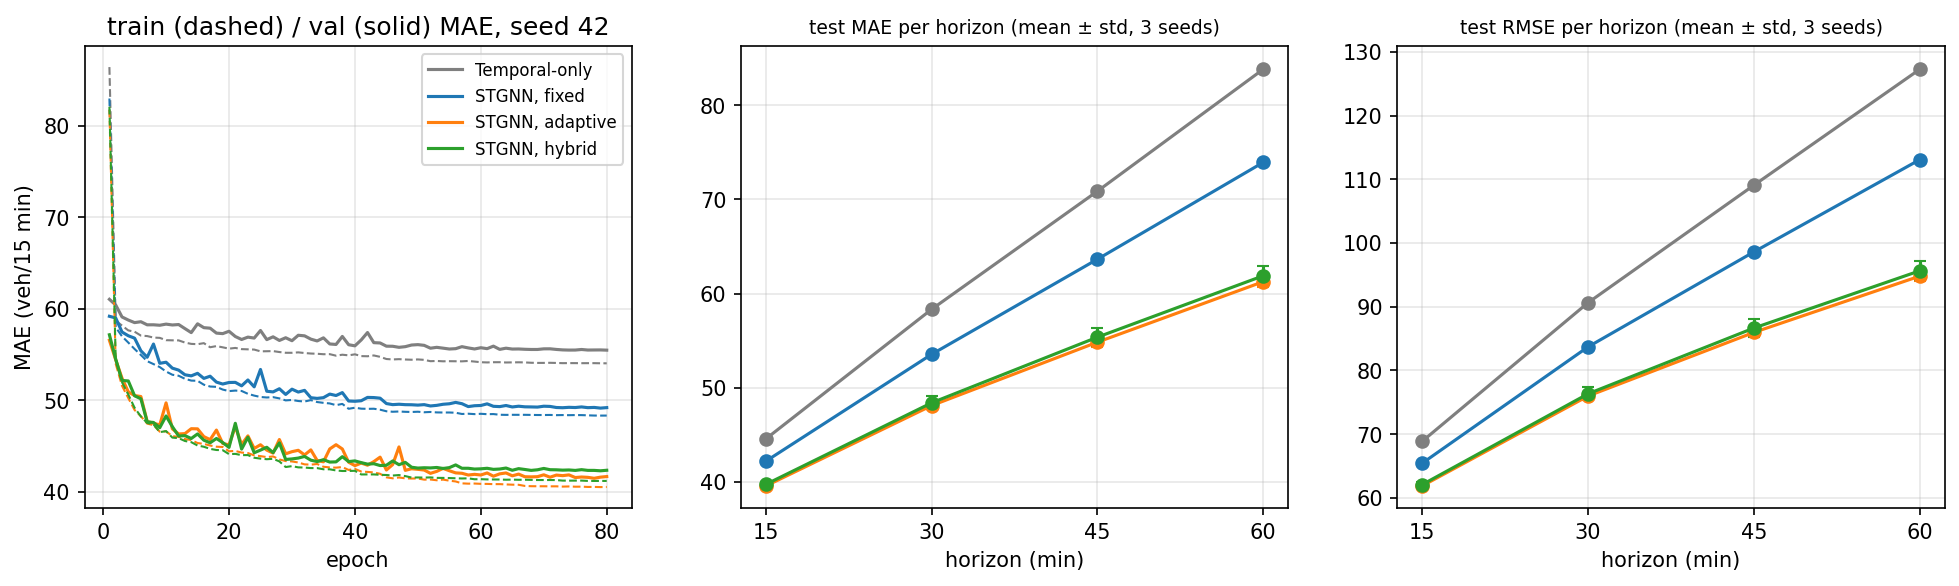
\includegraphics[width=\linewidth]{figures/q6a_curves_horizons.png}
  \caption{Learning curves (train dashed, validation solid) and test error per horizon.}
  \label{fig:curves}
\end{figure}

\begin{figure}[H]
  \centering
  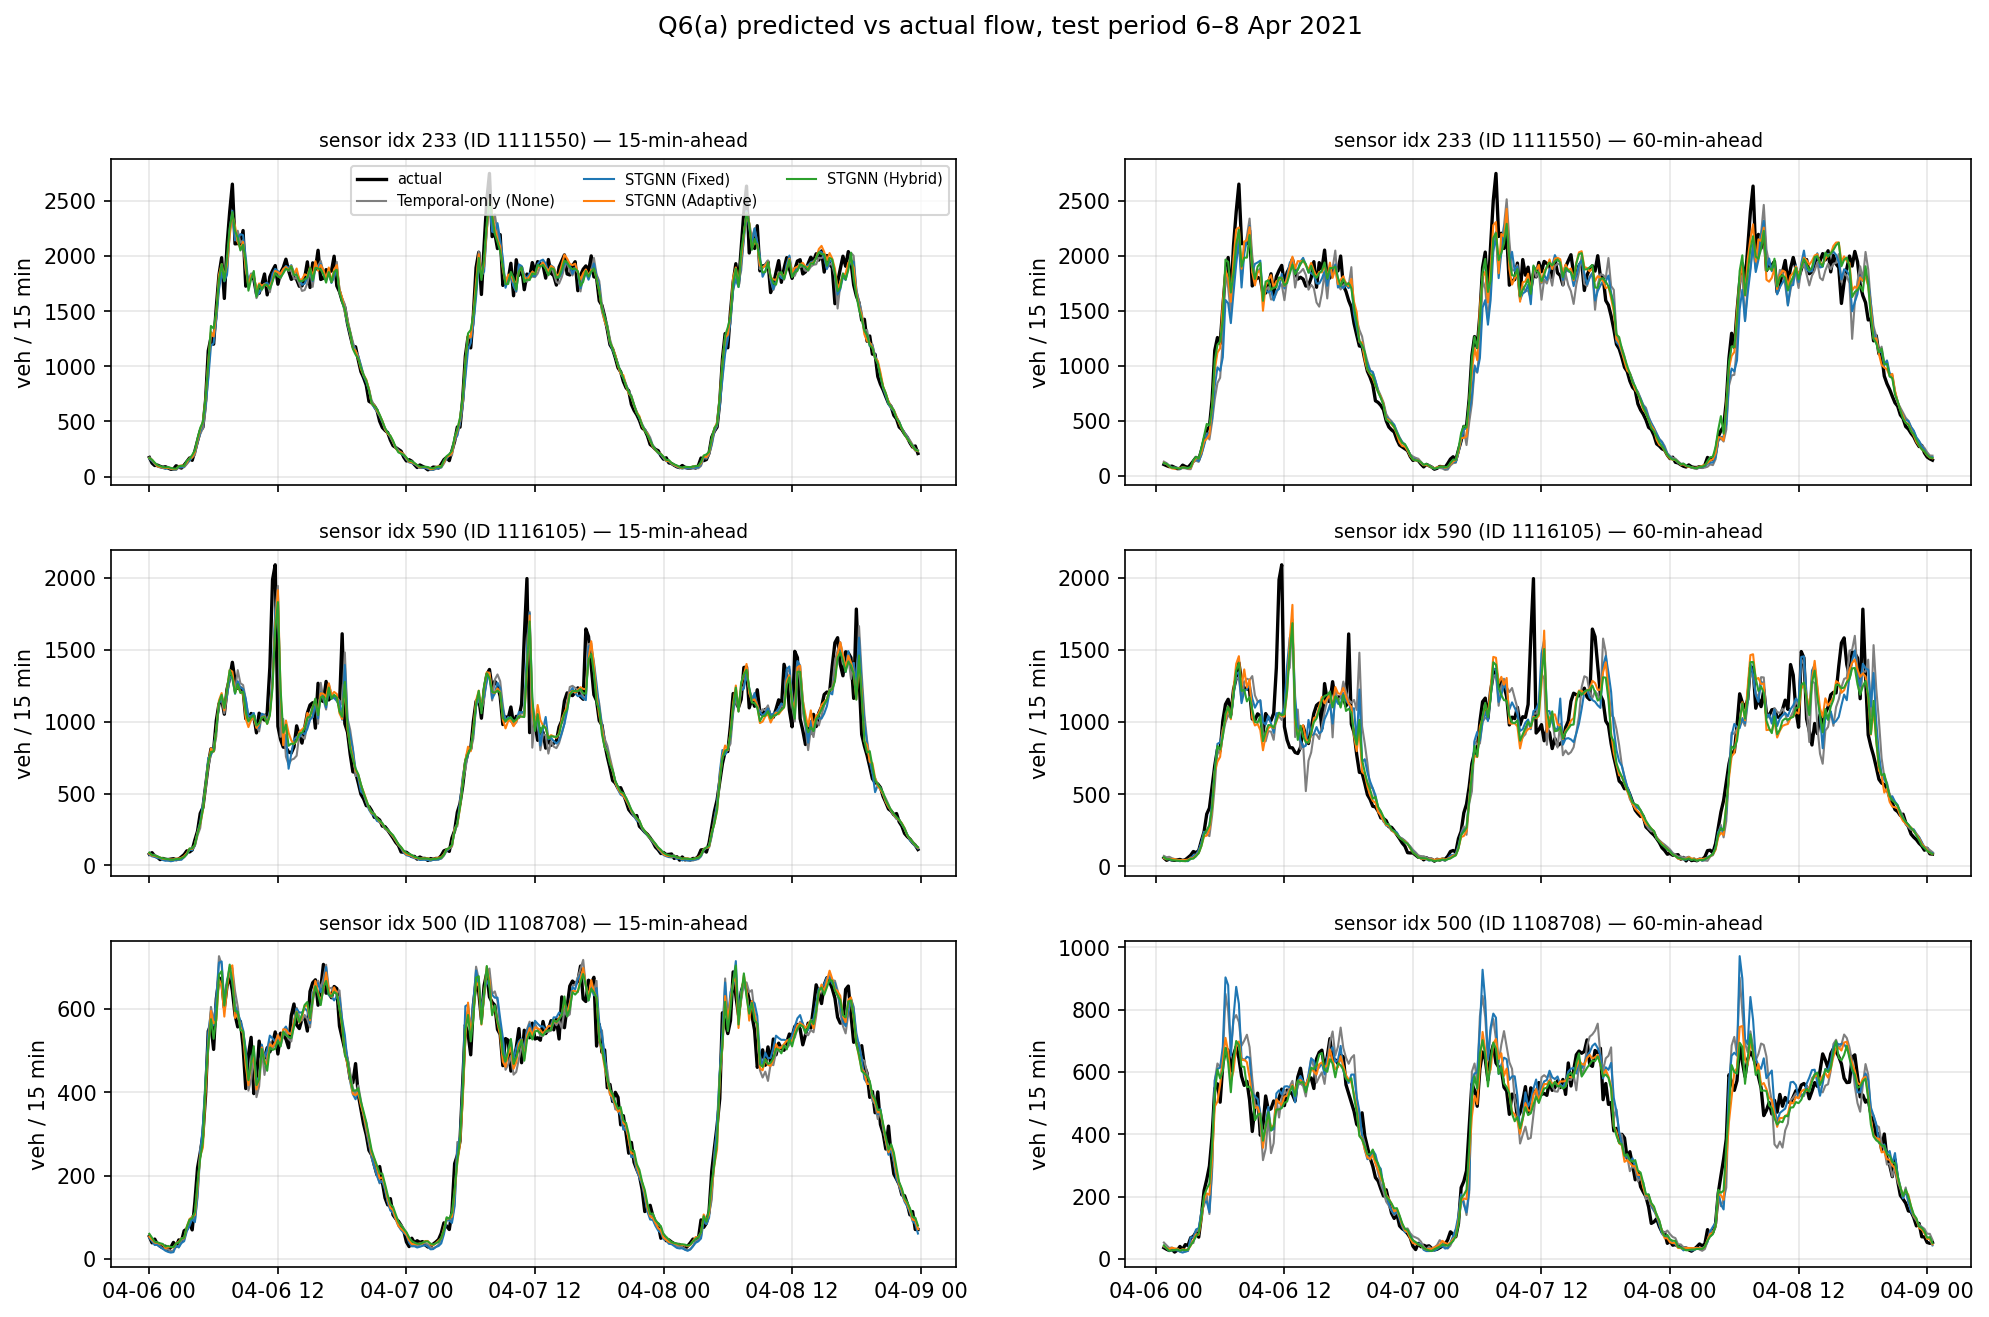
\includegraphics[width=\linewidth]{figures/q6a_pred_vs_actual.png}
  \caption{Predicted versus actual flow for three test sensors (I-8 W, SR-163 S, SR-78 W) during Tue 6 -- Thu 8 April 2021,
  15-minute-ahead (left) and 60-minute-ahead (right).}
  \label{fig:pred}
\end{figure}

\paragraph{Observations.}
(1) All learned models beat the naive references by a wide margin (last value: 87.1 MAE). (2) The ranking is
temporal-only $>$ fixed $>$ hybrid $\approx$ adaptive in error, on both validation and test, at every horizon.
(3) The value of spatial information grows with the horizon: the adaptive graph cuts 60-minute MAE by 25.7\% relative to
temporal-only, but 15-minute MAE by only 11.4\%. (4) In Figure~\ref{fig:pred}, all models follow the daily profile at
15\,min. At 60\,min the temporal-only and fixed models overshoot the morning ramp of sensor 500 by 200--300 veh/15\,min
(they extrapolate the rising trend), while the adaptive and hybrid models stay closer to the true plateau. No model
anticipates the sharp isolated spikes of sensor 590, which have no precursor in the 2-hour input. (5) Test errors are
about 15--22\% higher than validation errors for every model. The test period (Apr--Dec 2021) differs from the 2020
training year: it has more missing data (6.0\% vs 4.1\%) and, plausibly, traffic recovering from 2020 pandemic
conditions. The gap therefore most likely reflects distribution shift rather than overfitting (it appears for all models,
including the 6.5\,k-parameter baseline). (6) The adaptive model's best epoch was 49 of the 50-epoch cap,
so it might improve slightly with more epochs. Because the protocol must be identical for all models, we kept the cap.

\subsection{Q6(b) Graph structure analysis}\label{sec:q6b}
We compare the learned top-20 graph of the adaptive model with the road graph using (i) whether an edge exists in $A_{SD}$
and its hop distance in the (undirected) road graph, (ii) the straight-line (haversine) distance from the sensor coordinates,
and (iii) the Pearson correlation of the two sensors' \emph{2020} flow series. Uniformly random sensor pairs serve as the null
baseline.

\begin{table}[H]
\centering\small
\caption{Learned versus physical connectivity (adaptive model; ``top-$m$'' means each node's $m$ largest off-diagonal weights).}
\label{tab:graph}
\setlength{\tabcolsep}{4.5pt}
\begin{adjustbox}{max width=\linewidth}
\begin{tabular}{lrrrrrr}
\toprule
 & & \% road & \% within & median & median & mean 2020\\
Edge set & \# edges & edge & 2 hops & hops & km & corr.\\
\midrule
Road-graph edges            & 17\,319 & 100.0 & 100.0 & 1 & 2.4  & 0.855\\
Learned top-1 per node      & 716     & 7.4   & 17.0  & 6 & 19.3 & \textbf{0.903}\\
Learned top-5 per node      & 3\,580  & 5.8   & 13.8  & 7 & 21.2 & 0.881\\
Learned all kept (top-20)   & 14\,312 & 4.3   & 10.7  & 7 & 22.9 & 0.852\\
Hybrid (adaptive part) top-1 & 716    & 6.8   & 17.9  & 6 & 19.0 & 0.906\\
Random pairs                & 19\,970 & 4.1   & 9.8   & 7 & 23.1 & 0.842\\
\bottomrule
\end{tabular}
\end{adjustbox}
\end{table}

\begin{figure}[H]
  \centering
  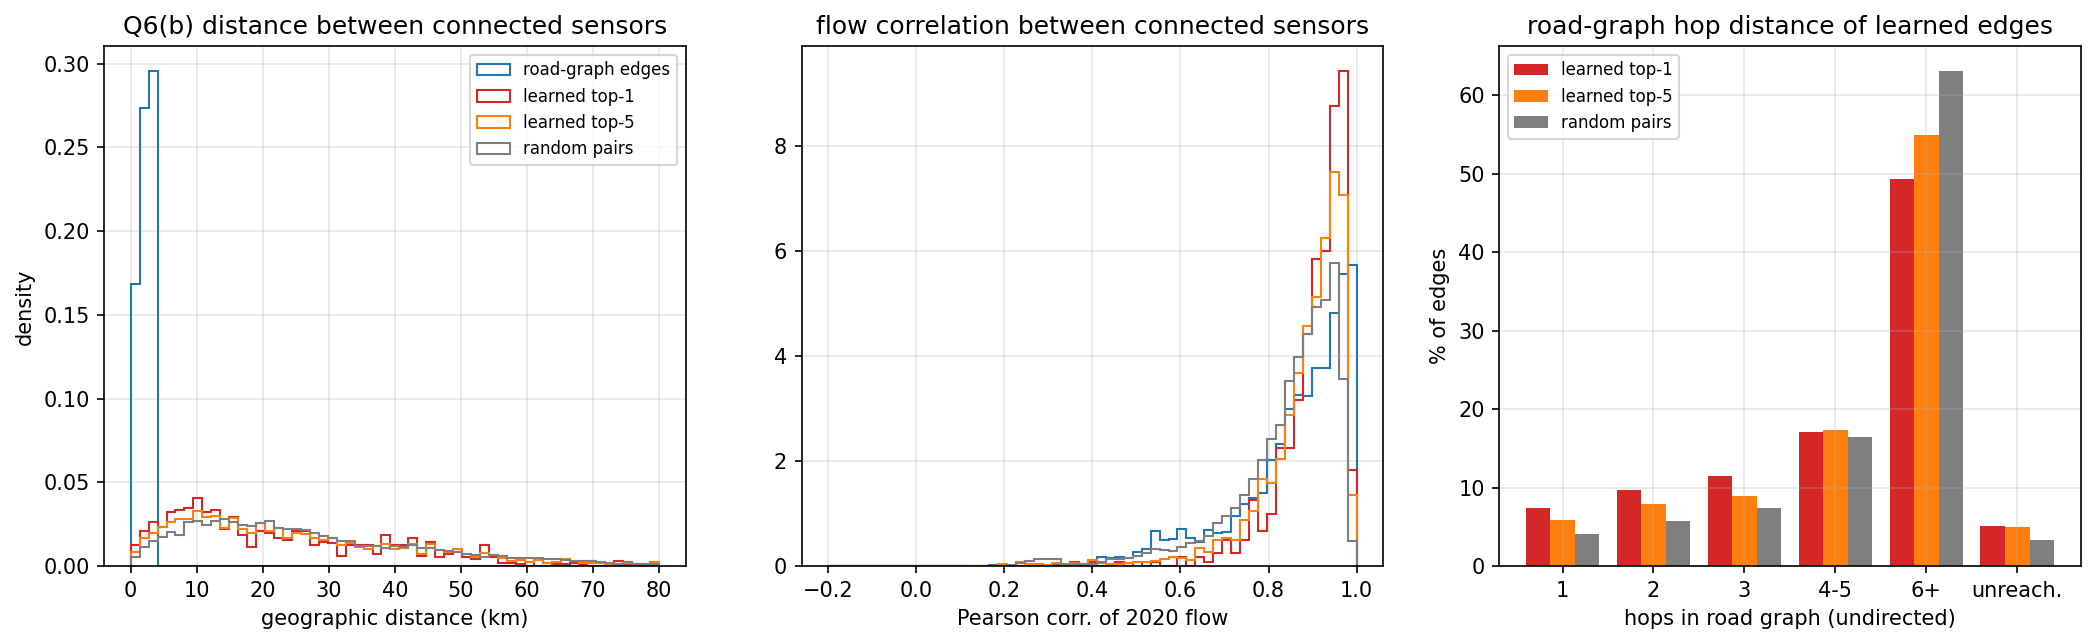
\includegraphics[width=\linewidth]{figures/q6b_learned_vs_physical.png}
  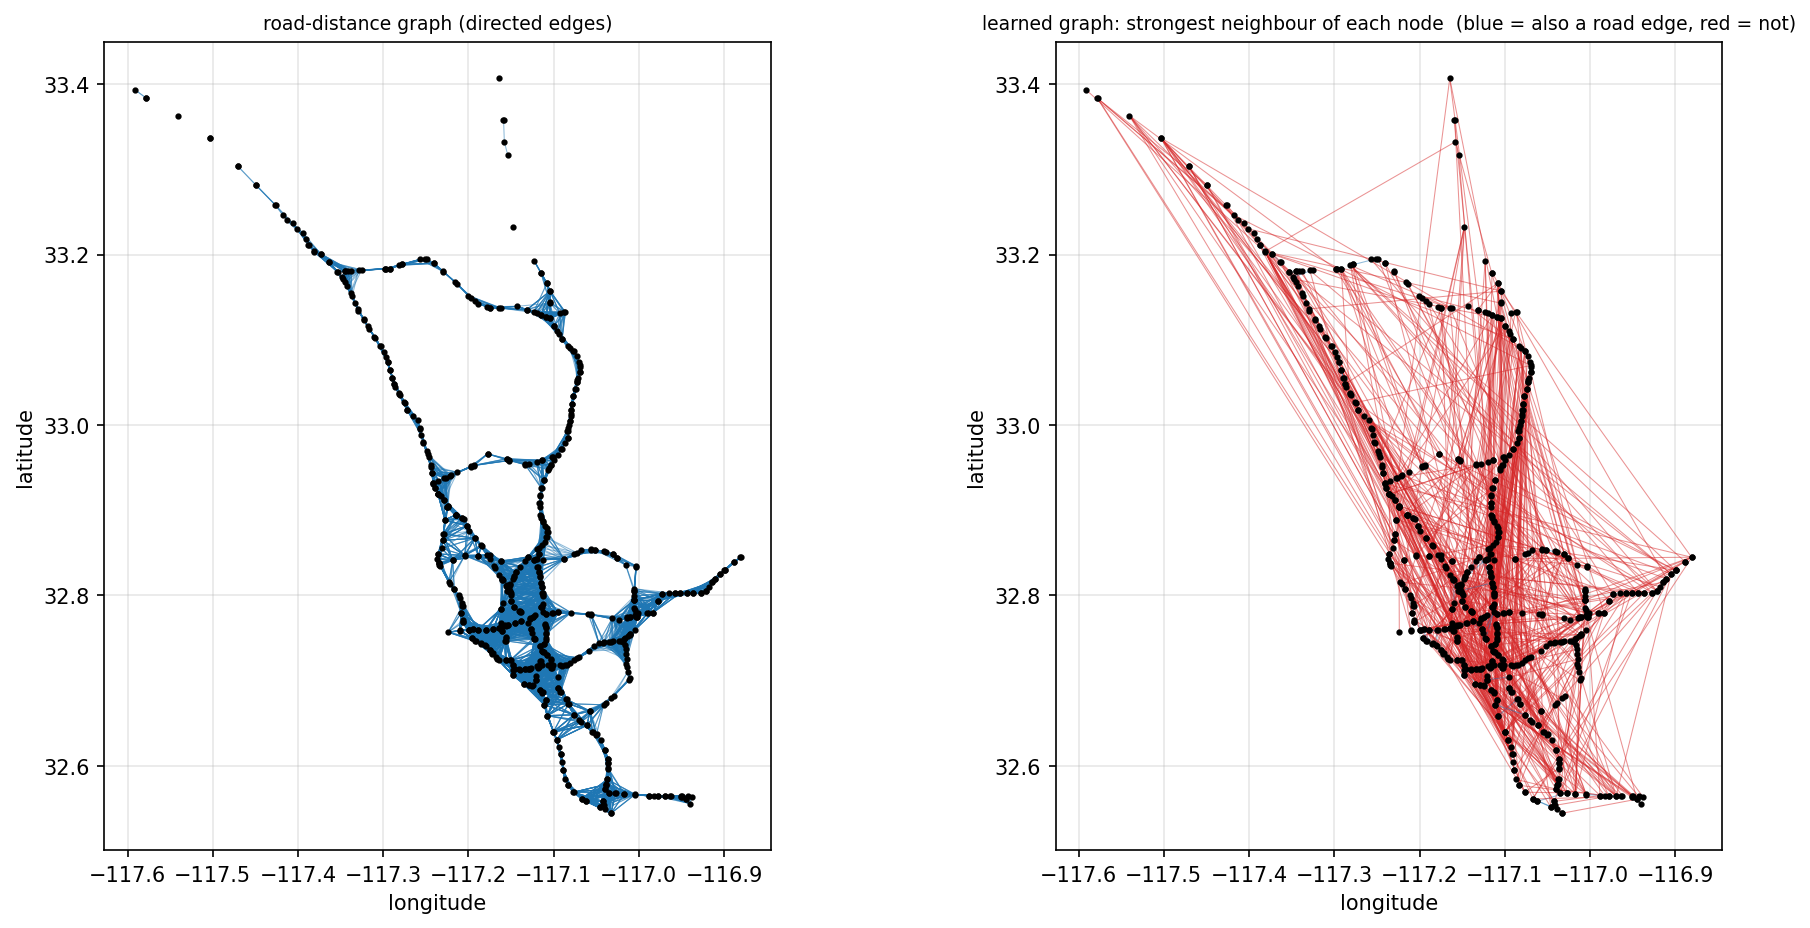
\includegraphics[width=0.92\linewidth]{figures/q6b_map_learned_edges.png}
  \caption{Q6(b). Top: distance distributions, flow-correlation distributions, and road-graph hop distance of learned
  edges compared with road edges and random pairs. Bottom: road graph (left) versus each sensor's strongest learned neighbour
  (right; blue = also a road edge, red = not).}
  \label{fig:q6b}
\end{figure}

\begin{enumerate}
\item \textbf{Are the strongest learned connections in the road graph?} Mostly not. Only 7.4\% of each node's strongest
learned neighbour is a road-graph edge (in either direction). That is $1.8\times$ the 4.1\% expected by chance, so there is a
weak enrichment, but more than 90\% of the strongest learned links are not physical edges. Among the 15 largest individual
weights, 4 are road edges (e.g.\ two co-located I-805 N/S sensors 0.13\,km apart, weight 0.92). The other 11 connect sensors
2--13 hops apart (median 9), and one pair is not connected in the road graph at all.
\item \textbf{Are learned connections geographically local?} Only weakly. Road-graph edges have a median length of 2.4\,km.
The learned top-1 edges have a median of 19.3\,km, close to the 23.1\,km of random pairs, and their distance histogram almost
matches the random one apart from a small excess below 15\,km. The share within 2 hops is 17\% versus 10\% for random pairs.
Locality emerges a little but is not what the model optimises for.
\item \textbf{Does the learned graph capture dependencies absent from the physical graph?} Yes. The learned top-1 neighbours
have a \emph{higher} mean 2020 flow correlation (0.903) than road neighbours (0.855) or random pairs (0.842), and the Spearman
correlation between learned weight and flow correlation on kept edges is 0.25. The model links sensors with similar temporal
profiles (same commuting direction and peak timing on different freeways) even when they are 20+\,km apart: a ``functional''
graph rather than a physical one. It also forms hub columns (484 of 716 nodes receive weight; the largest column sum is 9.4)
that act as shared reference profiles for many sensors. Some of the strongest weights point to sensors that had \emph{no}
observed 2020 data (their 2020 correlation is undefined). For these inputs the model sees a constant imputed series, so the
weight behaves like a learned bias rather than evidence of a traffic dependency.
\item \textbf{Why can a learned graph be better or worse than a fixed one?} \emph{Better}: it is optimised directly for the
forecasting loss. It can (a) connect sensors with similar daily or weekly patterns, which the encoder cannot otherwise
access because the model has no time-of-day input (neighbours effectively act as a learned temporal context), (b) bypass
missing or faulty neighbours, and (c) use sharper, task-specific weights instead of distance kernels in which a node averages
24 neighbours equally. \emph{Worse}: it has many more parameters ($N\times d_e\times2$), needs plenty of data and epochs, can
latch onto spurious correlations (as with the dead sensors), is not interpretable, and does not transfer to new sensors or a
changed network. The fixed graph encodes true causal propagation paths, which matter most for non-recurrent events
such as incidents, and it costs no parameters. With 35\,k training windows of strongly recurrent commuter traffic, the
data-driven graph wins here.
\end{enumerate}

\subsection{Q6(c) Critical discussion}
\begin{itemize}
\item \textbf{Does lower error imply the learned graph is the true road connectivity?} No. The adaptive graph has the lowest
error yet only 4--7\% of its edges are road edges, close to chance. Forecasting loss rewards any \emph{predictive} feature, and
correlation is not connectivity: two commuter routes 30\,km apart can share a peak time without any vehicle travelling between
them. The adjacency is also not identifiable. Many different $(E_1,E_2)$ and weight matrices $W_g$ give the same
predictions, and the GC weights, residual and head can compensate for a ``wrong'' graph. Some of the strongest weights
point to sensors with no training data at all. Learned graphs should be read as dependency or similarity structure, not as
a map.
\item \textbf{Why can a hybrid outperform either alone?} The two graphs carry complementary information. The physical graph is a
reliable prior for local, directional propagation (incidents, queue spill-back, missing-sensor smoothing) and helps early in
training and for rare events. The adaptive graph adds long-range similarity. A convex combination lets the model use the prior
where it helps and learn corrections elsewhere, and the prior regularises the embeddings. In our run the learned
$\alpha=0.057$, so the hybrid nearly reduced to the adaptive graph and performed the same (51.43 vs 51.34 MAE; slightly better
at 45--60\,min). This suggests that, for this recurrent-flow task and model, most of the spatial gain comes from learned
similarity. A hybrid would be expected to help more for congestion and speed forecasting, with fewer epochs, or under
distribution shift.
\item \textbf{Limitations of a static graph.} Traffic dependencies change during the day and the week. At 3\,a.m.\ sensors are
nearly independent and free-flowing. During the morning peak, inbound sensors couple strongly and queues propagate upstream
at shockwave speed, and the dominant direction reverses in the evening. Incidents, lane closures, weather and events
create short-lived dependencies, and 2020 lockdown patterns differ from 2021. A single matrix, fixed or learned, can only
capture an average of these regimes, so it over-smooths free-flow periods and under-represents peak-time propagation. Remedies
include time-varying or input-conditioned adjacency (e.g.\ attention over nodes, graphs that depend on time of day or the current
state, as in dynamic-graph STGNNs), separate forward and backward diffusion, and adding time-of-day/day-of-week features.
\end{itemize}

% ---------------------------------------------------------------------------
\section{Question 7 -- Reproducibility}
\paragraph{Code.} Everything is in one notebook, \texttt{notebook/dlstg\_pa3.ipynb} (generated from the jupytext source
\texttt{notebook/dlstg\_pa3.py}). The repository (\url{\repourl}) also contains:
\begin{itemize}
\item the executed notebook with all outputs (\texttt{notebook/dlstg\_pa3\_executed.ipynb});
\item the \texttt{outputs/} folder: figures, metrics (\texttt{results.json}, \texttt{results\_table.csv}), graph-analysis CSVs,
learned adjacency matrices, model weights and the run log;
\item \texttt{outputs.zip}, an archive of the same folder.
\end{itemize} The README gives step-by-step instructions to rerun on Kaggle (via the
Kaggle API or the web UI) or locally. If the dataset is not found, the notebook runs a small synthetic smoke test of the full
pipeline.

\paragraph{Hyper-parameters (identical for all four models).}
\begin{center}\small
\begin{tabular}{>{\raggedright\arraybackslash}p{0.30\linewidth}>{\raggedright\arraybackslash}p{0.62\linewidth}}
\toprule
Hyper-parameter & Value\\
\midrule
Input / output steps & 8 / 4 (15-minute steps)\\
Temporal encoder & Conv1d ($k$=3), Conv1d ($k$=3, dilation 2), Linear; hidden dim $d=32$\\
Graph convolution & 2 residual layers, $H \leftarrow H+\mathrm{ReLU}(\hat A H W)$\\
Forecast head & Linear(32,32), ReLU, Linear(32,4)\\
Fixed $\hat A$ & $D^{-1}\tilde A$ (directed random-walk normalisation)\\
Adaptive graph & embedding dim $d_e=10$, top-$k=20$ before row softmax\\
Hybrid $\alpha$ & learned, $\alpha=\sigma(a)$, initialised at 0.5\\
Loss & masked MAE on z-scored values\\
Optimiser & Adam, learning rate $10^{-3}$, no weight decay\\
Batch size & 64\\
Epochs & at most 50; early stopping with patience 8 on validation MAE\\
Gradient clipping & 5.0 (global norm)\\
Normalisation & z-score with mean/std of observed 2020 values\\
Random seed & \textbf{42} (Python, NumPy, PyTorch, CUDA)\\
Determinism & cuDNN deterministic mode; \texttt{CUBLAS\_WORKSPACE\_CONFIG=:4096:8}\\
\bottomrule
\end{tabular}
\end{center}
The parameter counts are 6\,500 (temporal-only), 8\,612 (fixed), 22\,932 (adaptive) and 22\,933 (hybrid). The seed is reset before
each model is built, so the shared modules start from the same initialisation. The epochs actually run and the best epochs are
listed in Table~\ref{tab:main}.

\paragraph{Hardware and timings.} The run was a Kaggle notebook (commit run): \textbf{1$\times$ NVIDIA Tesla T4 (15.6\,GB)}
(two were attached but only one was used), Intel Xeon @ 2.00\,GHz with 4 vCPUs, 33.7\,GB RAM, Linux 6.18, Python 3.13.16,
PyTorch 2.11.0+cu130 (CUDA 13.0), NumPy 2.1.3, pandas 2.3.3. Measured times: reading and extracting the two HDF5 years took
67\,s, and imputation under 1\,s. Training took 842\,s (temporal-only), 978\,s (fixed), 1063\,s (adaptive) and 1067\,s (hybrid),
i.e.\ 17.9--21.3\,s per epoch. The full notebook ran in about 70 minutes. The model is small enough to train on a CPU, but more
slowly.

\paragraph{Leakage checks.} Normalisation statistics, imputation profiles, the learned graphs and every trainable parameter use
training data only. The validation set is used only for early stopping, and all four models are evaluated on the same test
windows (April--December 2021) with the same mask.

% ---------------------------------------------------------------------------
\appendix
\section{Use of generative AI}
In line with the course AI policy, this section records how generative AI was used.

\paragraph{Tool.} Claude Code (Anthropic, model Claude Opus 5.5), an agentic coding assistant running in my terminal with
access to my local assignment folder, my Kaggle API credentials and the GitHub CLI.

\paragraph{Prompt (verbatim).}
\begin{quote}\small\ttfamily\raggedright
i have to do DLSTG\_PA3 instructions are in DLSTG\_PA3.pdf I want you to create a notebook and then use kaggle api to direcly run
it on kaggle and then do save and run and when the run is complete download the jupternotebook and the outputs zip file and
write the report also create a github respository and push everything on it with clean Readme to reproduce things if you have
any questions you can ask me
\end{quote}
Follow-up answers I gave to the assistant's questions: make the repository public now; use a Kaggle T4 GPU; write the report in
LaTeX and compile it to PDF; my name and roll number for the title page. I also downloaded the executed notebook and outputs
manually from Kaggle and asked the assistant to cross-check them against its own downloads (they are byte-identical).

\paragraph{Output.} The assistant (1) read the assignment PDF; (2) ran a small probe kernel on Kaggle to inspect the HDF5 layout,
the dataset mount path and the adjacency matrix; (3) wrote the notebook (Q1/Q2 numerical checks, data pipeline, models,
training and analysis), including a synthetic smoke-test mode, and tested it locally; (4) pushed it to Kaggle via the API on a
T4 GPU (the first push failed because the notebook lacked kernelspec metadata, and the second run succeeded); (5) downloaded the
executed notebook and outputs; (6) drafted this report, including the analytical answers to Q1--Q2 and the discussion, from
the measured outputs; and (7) created the GitHub repository and README.

\paragraph{Edits and verification.} All numbers in this report are copied from the executed notebook
(\texttt{outputs/results.json}, \texttt{outputs/graph\_analysis.csv}, \texttt{outputs/kaggle\_run\_log.txt}). Design choices
(sum aggregation, masked metrics, directed random-walk normalisation, top-$k$ before softmax) are justified in the relevant
sections. Any manual edits I make to the generated text before submission are listed here: none so far.

\end{document}
